%% 03-metode-pelaksanaan.tex — bab dokumen contoh prototipe-proposal (hal. 43-45 (proposal), hal. 45-46 (laporan)).
\chapter{METODE PELAKSANAAN}
\section{Pendekatan Perancangan}
\section{Lokasi dan Waktu}
\section{Prosedur Perancangan}

\begin{table}[htbp]
  \centering
  \caption{Ringkasan penelitian atau kegiatan terdahulu yang relevan}
  \label{tab:terdahulu}
  \begin{tabular}{clc}
    \toprule
    No & Fokus kajian & Hasil utama \\
    \midrule
    1 & Kajian pertama \citep{martin2014write} & Efektif pada ranah kognitif \\
    2 & Kajian kedua \citep{geraldi2017project} & Meningkat kategori sedang \\
    \bottomrule
  \end{tabular}
  \sumber{penulis dari berbagai sumber (2026)}
\end{table}

\begin{figure}[htbp]
  \centering
  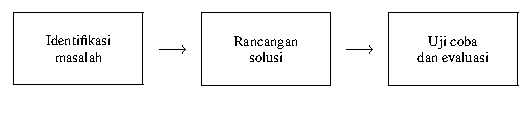
\includegraphics[width=8cm]{gambar/diagram-alur}
  \caption{Alur atau sketsa kegiatan}
  \label{gam:alur}
  \sumber{Dokumentasi penulis (2026)}
\end{figure}

\section{Teknik Perancangan}
\section{Teknik Uji Kelayakan Hasil}
Indikator capaian yang terukur di setiap tahapan disertakan pada subbab ini.
